% !TeX root = ../praktikum.tex
% !TeX encoding = UTF-8
% !Tex spellcheck = de_DE

Die geometrische Optik ist der Teilbereich der Optik, wo Lichtwellen durch idealisierte Strahlen angenähert werden um den Weg des Lichtes zu (re)konstruieren. Sämtliche Schlussfolgerungen basieren auf diesen vier Axiomen:

\begin{enumerate}
	\item{Axiom:} In homogenem Material verlaufen Lichtstrahlen gerade.
	\item{Axiom:} An der Grenze zwischen zwei homogenen und isotropen Materialien wird das Licht nach dem Reflexionsgesetz reflektiert und nach dem Brechungsgesetz gebrochen.
	\item{Axiom:} Zeit- bzw. Strahlenumkehr, die Richtung eines Lichtstrahles ist belanglos.
	\item{Axiom:} Die Lichtstrahlen beeinflussen sich nicht gegenseitig.
\end{enumerate}

Durch die spezielle Geometrische Form von Sammellinsen ergibt sich ein Brechungswinkel in Abhängigkeit vom Abstand zum Mittelpunkt, der effektiv Strahlen bündeln oder kollimieren kann. Die Brennweite gibt den Abstand an, in dem sich eine punktförmige Lichtquelle befinden muss, um von der Linse kollimiert zu werden. Gleichzeitig ist sie auch die Entfernung in der ein kollimierter Strahl hinter einer Linse gebündelt wird (siehe auch drittes Axiom).

Neben den Effekten der geometrischen Optik gibt es noch Effekte, die sich nicht durch dieses einfache Modell beschreiben lassen. Hierzu zählt die Streuung. Diese kann nach dem Huygenssches Prinzip\cite{} beschrieben und mittels der Beschreibung durch die Frauenhoferbeugung\cite{} vereinfacht werden. Die wesentliche Erkenntnis hieraus ist, dass ein Lichtstrahl an einem Spalt, der in der Größenordnung der Wellenlänge liegt,

Es kann nun gezeigt werden, dass eine Sammellinse eine einfallende ebene Welle derart verändert, dass die Amplitudeninformation einer FT unterworfen wird. Dies ist in Abbildung~\ref{fig:ft-an-linse} am Beispiel eines Spaltes illustriert. Eine mathematische Herleitung ist zum Beispiel im Begleitheft zu diesem Versuch oder in \cite{bibid} zu finden.

\begin{figure}[h]
	\centering
	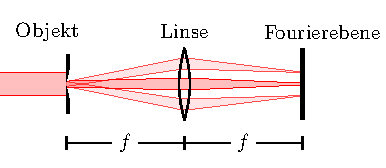
\includegraphics[scale=1]{graphs/theorie/ft-an-linse.pdf}
	\caption[Illustration: Fouriertransformation an einer Linse]{
		Ein kollimierter Laserstrahl von Links trifft auf ein Objekt (hier einen Spalt) und wird gestreut. Hier sind beispielhaft drei Strahlenverläufe eingezeichnet. Man erkennt, dass durch das Objekt die Intensitätsverteilung in der Fourierebene beeinflusst wird.
	} \label{fig:ft-an-linse}
\end{figure}